\documentclass[runningheads]{llncs}

% ---------------------------------------------------------------
% Include basic ACCV package
\PassOptionsToPackage{table,dvipsnames}{xcolor}
% TODO REVIEW: Insert your submission number below by replacing '*****'
% TODO FINAL: Comment out the following line for the camera-ready version
\usepackage[review,year=2026,ID=230]{accv}
% TODO FINAL: Un-comment the following line for the camera-ready version
%\usepackage{accv}

% ---------------------------------------------------------------
% Other packages
\usepackage{accvabbrv}
\usepackage{graphicx}
\usepackage{booktabs}
\usepackage{amsmath,amssymb,amsfonts}
\usepackage{tikz}
\usetikzlibrary{arrows.meta,positioning,fit,calc,shapes.geometric}
\usepackage{adjustbox}
\usepackage{siunitx}
\usepackage{array}
\usepackage{multirow}
\usepackage{enumitem}
% \usepackage[accsupp]{axessibility}  % uncomment if package available

% TODO FINAL: Comment out the following line for the camera-ready version
\usepackage[pagebackref,breaklinks,colorlinks,citecolor=accvblue]{hyperref}
% TODO FINAL: Un-comment the following line for the camera-ready version
%\usepackage{hyperref}
% \usepackage{orcidlink}  % uncomment if package available

% ---- Layout tweaks ----
\usepackage[skip=4pt]{caption}
\setlength{\textfloatsep}{8pt plus 2pt minus 2pt}
\setlength{\intextsep}{6pt plus 2pt minus 2pt}
\setlength{\emergencystretch}{2em}
\newcommand{\tabtight}{\setlength{\tabcolsep}{3.5pt}\renewcommand{\arraystretch}{1.10}}

% ---- Convenience macros ----
\newcommand{\TDS}{\textsc{TDS}}

% ---- Revision marking (rebuttal round) ----------------------------------
% Every change made in response to the reviews is wrapped in \rev{...} so the
% revised text is legible as a diff. \revdel{...} keeps deleted text visible,
% struck through, where seeing what went is more informative than its absence.
% For the camera-ready, redefine both to be invisible:
%     \renewcommand{\rev}[1]{#1}
%     \renewcommand{\revdel}[1]{}
\usepackage{xcolor}
\usepackage[normalem]{ulem}  % normalem: do not hijack \emph
\definecolor{revblue}{RGB}{0,80,200}
\newcommand{\rev}[1]{\textcolor{revblue}{#1}}
\newcommand{\revdel}[1]{\textcolor{gray}{\sout{#1}}}

\begin{document}
\raggedbottom

% ---------------------------------------------------------------
% Revised title. "Mitigating" is dropped: the only mitigation result was a
% confidence cascade whose gain does not survive held-out calibration.
% "Aliasing" becomes "Sampling Sensitivity" because, as R2 and R3 argue and we
% confirm in Sec. 3.2, the protocol varies evidence available to the model
% rather than the sampling rate of the underlying signal.
\title{\rev{Measuring Spatiotemporal Sampling Sensitivity in Video Action
Recognition: A Cross-Architecture Analysis at Scale}}

\titlerunning{\rev{Spatiotemporal Sampling Sensitivity in Video Action Recognition}}

\author{Anonymous ACCV Submission}
\authorrunning{Anonymous Submission}
\institute{}
\maketitle

% =========================================================
\begin{abstract}
Temporal resolution in video action recognition is usually treated as a fixed hyperparameter rather than a sampling constraint. We present a large-scale study of empirical classifier-evidence loss under temporal and spatial subsampling across 8 architectures and 8 datasets. \rev{We first characterise what a strided sampling protocol actually varies: because strided candidates are re-uniformised to a model's fixed frame budget, stride alters the input only once the candidate pool falls below that budget. The resulting sensitivity therefore measures how much distinct evidence a model receives, not the sampling rate of the underlying signal, and it is gated by the ratio of clip length to frame budget (Spearman $0.96$ against dataset-level sensitivity).} \revdel{Within this evaluated pool, aliasing sensitivity varies systematically across temporal aggregation designs, as certain sequence models and divided-attention Transformers suffer 3--5$\times$ less degradation under frame reduction compared to standard Convolutional Neural Networks (CNNs).} \rev{Controlling for this by supplying every architecture the same distinct frames at the same positions, an architecture effect survives in a narrower form: divided-attention and state-space designs deliver more accuracy per distinct frame (Spearman $0.82$, $p=0.02$ against the uncontrolled ordering), though the previously reported 3--5$\times$ magnitude does not.} We introduce the \textbf{Temporal Demand Score (\TDS{})} to quantify accuracy loss under temporal subsampling\rev{; its dataset ranking is invariant to curve-integral, unclipped and baseline-normalised definitions}\revdel{ which has demonstrated that fine-grained sports demand as much temporal density as sign language}. In a cross-resolution evaluation, CNNs degrade at novel resolutions without fine-tuning, whereas Transformers natively maintain accuracy\rev{; we separate the gain from target-resolution adaptation ($\approx$32pp) from the gain due to additional training alone ($\approx$7pp)}. Furthermore, hardware profiling shows video state-space models are 4--8$\times$ slower than efficient Transformers. \revdel{To optimize deployment, we demonstrate an entropy-based adaptive frame routing cascade that halves temporal budgets without accuracy loss.} \rev{A maximum-probability confidence cascade traces a lower-frame operating point, which we report with held-out calibration as a deployment illustration rather than a mitigation method.} Finally, we provide a reproducibility package and an interactive visualization dashboard\rev{, and we release the diagnostic that identifies, for any dataset and frame budget, the stride at which a fixed-budget pipeline degenerates}.
\keywords{\rev{Temporal sampling} \and Video recognition \and \rev{Evidence loss}}
\end{abstract}

% =========================================================
\section{Introduction}
\label{sec:intro}

Applications of activity recognition include driving, healthcare, and surveillance~\cite{5771372,10484402}. The field has evolved from 3D ConvNets and dual-pathway networks~\cite{tran2015c3d,carreira2017i3d,tran2018r2plus1d,wang2018nonlocal,feichtenhofer2019slowfast} to video Transformers and state-space models~\cite{bertasius2021timesformer,arnab2021vivit,liu2022videoswin,fan2021mvit,tong2022videomae,wang2023videomaev2,li2024videomamba}.

Despite this diversity, all models are evaluated using standardized sampling recipes (8--32 uniformly-sampled frames at fixed stride), treating temporal resolution as a static implementation detail. This assumption fails in real-world deployments where constraints on computational hardware, power usage, sensor capabilities, or communication bandwidth make dense sampling infeasible~\cite{lin2019tsm}. This leaves two fundamental questions unanswered: \emph{when} does temporal subsampling become destructive, and \emph{why} do different architectures respond differently?

\paragraph{Sampling perspective.}
The Nyquist--Shannon theorem~\cite{shannon1949communication} motivates the intuition that undersampling can distort a temporal signal rather than merely compress it, a principle also relevant to perception~\cite{vanrullen2007wagon} and deep learning~\cite{zhang2019antialiased}. \rev{We initially adopted this as a conceptual guide. We now state a sharper limitation, because it shapes how every temporal result below must be read: when a recogniser consumes a fixed number of frames, the realised sampling rate is that number divided by the observed span, so no frame-subsampling protocol can vary sampling rate without simultaneously varying the evidence available or the temporal context. Aliasing in the signal-processing sense is therefore \emph{not identifiable} from such a sweep, and we do not claim to measure it. What we measure, and what the} \TDS{} \rev{metric quantifies, is empirical classifier-evidence loss under controlled subsampling. To test the stronger reading directly rather than assume it away, we additionally report an intervention that holds the frame count and span fixed and low-pass filters the clip before sampling, which is the condition under which genuine aliasing --- and only genuine aliasing --- would be recovered (Sec.~\ref{sec:results_temporal}).}\revdel{ We use this as a conceptual guide, but introduce an empirical Temporal Demand Score (\TDS{}) metric that measures how much classifier evidence is lost under controlled subsampling, not literal spectral aliasing of the raw video signal.}

\begin{figure}[t]
\centering
\begin{adjustbox}{max width=\columnwidth}
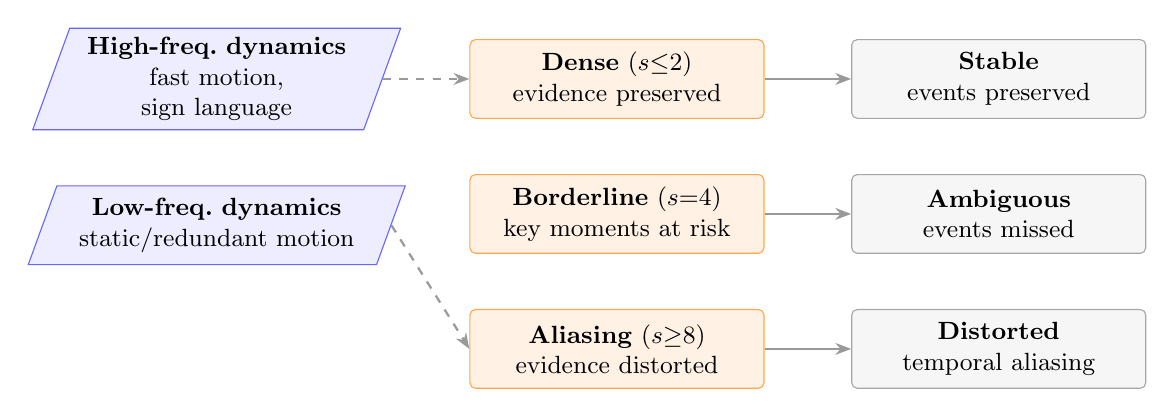
\begin{tikzpicture}[font=\small, node distance=7mm]
\tikzset{
  act/.style  ={draw, trapezium, trapezium left angle=70,
                trapezium right angle=110, align=center, minimum height=1.0cm, text width=3.5cm, fill=blue!7, draw=blue!60},
  samp/.style ={draw, rounded corners=2pt, align=center,
                minimum height=1.0cm, text width=3.5cm, fill=orange!10, draw=orange!70},
  obs/.style  ={draw, rounded corners=2pt, align=center,
                minimum height=1.0cm, text width=3.5cm, fill=gray!7, draw=gray!70},
  aI/.style={-{Stealth[length=2mm]},thick,dashed,draw=gray!80},
  aO/.style={-{Stealth[length=2mm]},thick,draw=gray!80}
}
\node (hf)[act]{\textbf{High-freq.\ dynamics}\\fast motion, sign language};
\node (lf)[act,below=of hf]{\textbf{Low-freq.\ dynamics}\\static/redundant motion};
\node (d)[samp,right=11mm of hf]{\textbf{Dense} ($s{\leq}2$)\\evidence preserved};
\node (n)[samp,below=of d]{\textbf{Borderline} ($s{=}4$)\\key moments at risk};
\node (a)[samp,below=of n]{\textbf{Aliasing} ($s{\geq}8$)\\evidence distorted};
\node (o1)[obs,right=11mm of d]{\textbf{Stable}\\events preserved};
\node (o2)[obs,below=of o1]{\textbf{Ambiguous}\\events missed};
\node (o3)[obs,below=of o2]{\textbf{Distorted}\\temporal aliasing};
\draw[aI](hf.east)--(d.west); \draw[aI](lf.east)--(a.west);
\draw[aO](d.east)--(o1.west); \draw[aO](n.east)--(o2.west); \draw[aO](a.east)--(o3.west);
\end{tikzpicture}
\end{adjustbox}
\caption{Temporal aliasing as empirical evidence loss: sparse sampling can miss or distort the frames a recognizer needs, especially for temporally localized actions.}
\label{fig:aliasing_concept}
\end{figure}

\paragraph{Contributions.}
We conduct a systematic cross-architecture study of spatiotemporal aliasing:
\begin{enumerate}[leftmargin=*,topsep=2pt,itemsep=1pt]
\item \textbf{Temporal Demand Score (\TDS{})}: an architecture-averaged metric that measures a dataset's aliasing sensitivity. We demonstrate its utility by ranking 8 diverse datasets with leave-one-architecture-out analysis, architecture-family ablation (CNN-only, Transformer-only), and bootstrap confidence intervals checking ranking stability (Sec.~\ref{sec:results_tds}; supplementary material). 
% FineGym (55.9pp) rivals sign language (AUTSL, 53.0pp) as the highest-demand domain.
\item \textbf{Cross-architecture aliasing characterization}: 8,000 core evaluation
configurations show strong empirical architecture-level differences within our pool, with VideoMamba and TimeSformer losing 3--5$\times$ less accuracy under stride stress than CNNs and ViViT; this is an association, not a controlled temporal-module ablation (Sec.~\ref{sec:results_temporal}).
\item \textbf{Target-resolution fine-tuning}: Fine-tuning each model at the target spatial resolution closes the cross-resolution gap by up to 39pp for CNNs. In contrast, Transformers naturally maintain accuracy across different image sizes and require no retraining (Sec.~\ref{sec:results_spatial})
\item \textbf{Measured inference latency}: GPU latency characterization
across all 8 models $\times$ 5 target resolutions (bfloat16), enabling sampling-aware deployment budgeting per device class (Sec.~\ref{sec:results_latency}).
\item \textbf{Practical illustration and reproducibility package}: as a low-cost downstream use of the temporal-sweep results above---rather than a new routing algorithm---a simple entropy-threshold cascade traces a validation Pareto frontier with 52\% fewer frames on the Something-Something (SSv2) temporal dataset while matching dense-sampling accuracy. We also provide a supplementary package containing a deterministic dashboard, evaluation scripts, and result tables; public code will be released after review (Sec.~\ref{sec:results_routing}).
\end{enumerate}

% =========================================================
\section{Related Work}
\label{sec:related}

\subsection{Video Recognition Architectures}

\textbf{CNN-based architectures.} 3D ConvNets learn spatiotemporal features end-to-end~\cite{tran2015c3d,carreira2017i3d}, while Non-local Networks introduce global self-attention~\cite{wang2018nonlocal}. Factorized variants such as R(2+1)D and MC3 improve optimization and efficiency~\cite{tran2018r2plus1d,tran2019video}; SlowFast processes two frame-rate streams simultaneously~\cite{feichtenhofer2019slowfast}.

\textbf{Transformer and SSM architectures.} Video Transformers extend patch-based recognition to time: TimeSformer uses divided space-time attention~\cite{bertasius2021timesformer}, ViViT uses factorized attention~\cite{arnab2021vivit}, and VideoMAE learns via masked patch reconstruction~\cite{tong2022videomae,wang2023videomaev2}. VideoMamba~\cite{li2024videomamba} brings selective state-space scanning~\cite{gu2023mamba,dao2024mamba2} to video. Prior robustness work benchmarks spatial and photometric corruptions~\cite{schiappa2023robustness}; we instead isolate temporal and spatial sampling effects across this architectural spectrum.

\subsection{Temporal Sampling and Adaptive Inference}

Efficient inference methods sample or process fewer frames. TSN and TSM define sparse-sampling recipes~\cite{wang2016tsn,lin2019tsm}; AdaFrame selects frames~\cite{wu2019adaframe}; AdaFocus crops regions~\cite{wang2021adafocus}; AR-Net adapts resolution~\cite{meng2020arnet}; and FrameExit uses confidence cascades~\cite{ghodrati2021frameexit}. Dataset-level temporal reasoning has been studied with shuffled frames~\cite{huang2018makes} and motion-only cues~\cite{sevilla2021only}. These works do not measure the accuracy cliff induced by controlled stride and coverage sweeps; our \TDS{} metric provides an architecture-averaged temporal-demand ranking.

\subsection{Sampling Theory in Deep Learning}

Sampling theory predicts that undersampling a signal below its highest temporal frequency creates aliasing~\cite{shannon1949communication}. Temporal aliasing is well documented in perception~\cite{vanrullen2007wagon}; in deep learning, strided operators can violate shift-invariance unless anti-aliased~\cite{zhang2019antialiased}. Frequency-domain analysis has been explored for action recognition~\cite{tran2014frequency}, but not as a large-scale cross-architecture stress test of modern video models.

% =========================================================
\section{Methodology}
\label{sec:method}

\begin{figure*}[t]
\centering
\resizebox{\textwidth}{!}{%
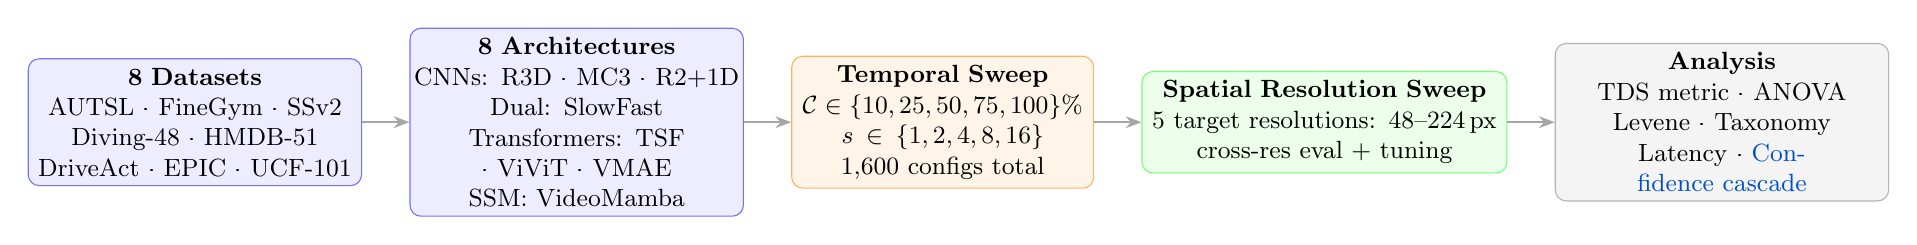
\begin{tikzpicture}[node distance=7mm,font=\small]
\tikzset{
  data/.style={draw,rounded corners,align=center,minimum height=8mm,text width=3.6cm,fill=blue!7,draw=blue!55},
  proc/.style={draw,rounded corners,align=center,minimum height=8mm,text width=3.6cm,fill=orange!9,draw=orange!60},
  p3/.style={draw,rounded corners,align=center,minimum height=8mm,text width=3.6cm,fill=green!8,draw=green!55},
  eval/.style={draw,rounded corners,align=center,minimum height=8mm,text width=4.0cm,fill=gray!9,draw=gray!60},
  arr/.style={-{Stealth[length=2mm]},thick,draw=gray!70}
}
\node(ds)[data,text width=4.0cm]{\textbf{8 Datasets}\\AUTSL · FineGym · SSv2\\Diving-48 · HMDB-51\\DriveAct · EPIC · UCF-101};
\node(ar)[data,right=6mm of ds,text width=4.0cm]{\textbf{8 Architectures}\\\makebox[\linewidth]{CNNs: R3D · MC3 · R2+1D}\\Dual: SlowFast\\Transformers: TSF · ViViT · VMAE\\SSM: VideoMamba};
\node(e1)[proc,right=6mm of ar]{\textbf{Temporal Sweep}\\$\mathcal{C}\in\{10,25,50,75,100\}\%$\\$s\in\{1,2,4,8,16\}$\\1,600 configs total};
\node(e6)[p3,right=6mm of e1, text width=4.4cm]{\textbf{Spatial Resolution Sweep}\\5 target resolutions: 48--224\,px\\cross-res eval + tuning};
\node(an)[eval,right=6mm of e6]{\textbf{Analysis}\\TDS metric · ANOVA\\Levene · Taxonomy\\Latency · \rev{Confidence cascade}};
\draw[arr](ds)--(ar); \draw[arr](ar)--(e1); \draw[arr](e1)--(e6); \draw[arr](e6)--(an);
\end{tikzpicture}}
\caption{Pipeline: the core factorial sweep uses 8 architectures $\times$ 8 datasets $\times$ 5 target resolutions (48--224px) $\times$ 5 coverages $\times$ 5 strides = \textbf{8,000 configurations}.}
\label{fig:pipeline}
\end{figure*}

\subsection{Datasets and Architectures}

Table~\ref{tab:datasets} summarizes the 8 datasets selected to span semantic domains, motion frequencies, and recording conditions. We evaluate 8 architectures from four families: (i) \textbf{3D CNNs}: R3D-18, MC3-18~\cite{tran2019video}, R(2+1)D-18~\cite{tran2018r2plus1d}; (ii) \textbf{dual-pathway}: SlowFast-R50~\cite{feichtenhofer2019slowfast}; (iii) \textbf{Transformers}: TimeSformer~\cite{bertasius2021timesformer}, ViViT~\cite{arnab2021vivit}, VideoMAE~\cite{tong2022videomae}; (iv) \textbf{SSM}: VideoMamba~\cite{li2024videomamba}. All models are fine-tuned from Kinetics-400 checkpoints using AdamW with cosine decay. We use fixed validation clip lists across models (approximately 20 clips/class, or all available clips for smaller classes); additional split, crop, seed, and frame-normalization details are in the supplementary material.

\begin{table}[t]
\centering
\caption{\TDS{} = mean accuracy drop (stride=1$\to$16, cov=100\%) per Eq.~\ref{eq:tds}, averaged over all 8 architectures ($n{=}8$). Sorted by \TDS{}. \textbf{Bold} = the two co-equal highest-demand domains (their relative order is leave-one-out sensitive; ranks 3--8 are stable under the supplementary robustness analysis).}
\label{tab:datasets}
\scriptsize\tabtight
\begin{tabular}{l r r l r r}
\toprule
Dataset & Classes & Videos & Domain & \TDS{} & $n$ \\
\midrule
FineGym~\cite{shao2020finegym}       &  97 & 1,960 & Fine-grained sport & \textbf{55.9pp} & 8 \\
AUTSL~\cite{sincan2020autsl}         & 226 & 4,418 & Sign language      & \textbf{53.0pp} & 8 \\
SSv2~\cite{goyal2017ssv2}            & 174 & 3,464 & Causal/temporal    & 27.6pp          & 8 \\
DriveAct~\cite{martin2019driveact}   &  33 &   448 & In-vehicle         & 21.9pp          & 8 \\
Diving-48~\cite{li2018diving48}      &  48 &   743 & Fine-grained       & 19.2pp          & 8 \\
HMDB-51~\cite{kuehne2011hmdb}        &  51 &   885 & Sports             & 16.6pp          & 8 \\
EPIC-Kitchens~\cite{damen2022epic}   &  89 & 1,020 & Egocentric         &  9.7pp          & 8 \\
UCF-101~\cite{soomro2012ucf101}      & 101 & 2,020 & Appearance         &  4.9pp          & 8 \\
\bottomrule
\end{tabular}
\end{table}

\subsection{Temporal Sampling Protocol}

We decouple \textit{temporal coverage} $\mathcal{C}$ (fraction of clip observed) from \textit{temporal stride} $s$ (sampling density), forming a 5$\times$5 grid: $\mathcal{C}\in\{10,25,50,75,100\}\%$ and $s\in\{1,2,4,8,16\}$. The temporal sweep at native resolution yields $8{\times}8{\times}25{=}\mathbf{1{,}600}$ model--dataset--configuration triples. Repeating this grid at the 5 target resolutions from 48--224px yields the \textbf{8,000} core configurations.

\paragraph{Coverage implementation.}
Coverage is applied from the \emph{beginning} of each clip: the first $\lfloor T\cdot\mathcal{C}/100\rfloor$ frames form the candidate pool, and $s$ \revdel{controls sampling density within that window}\rev{decimates it}. This simulates a sensor that observes only a leading fraction of the action and gives the sharpest measurement of how early the model has enough temporal context. Random window placement would confound temporal structure with missing-data effects.

\rev{\paragraph{What the stride axis varies.}
Because every architecture consumes a fixed number of frames $B$, the decimated candidate pool is re-uniformised to length $B$ before it reaches the model. Two consequences follow, and both matter for interpreting Sec.~\ref{sec:results_temporal}. First, whenever $\lceil \mathcal{C}T/100s\rceil \geq B$ the selected frames still span the same window with essentially the same spacing, so $s$ leaves the input nearly unchanged: on UCF-101 at $\mathcal{C}=100\%$ the median interval between sampled frames is $0.395$s at $s=1,2,4$ \emph{and} $8$. Second, once the pool falls below $B$ the shortfall is filled by repeating the final candidate, so the model receives $\lceil \mathcal{C}T/100s\rceil$ distinct frames followed by a static tail.

The temporal axis of our sweep is therefore a measure of \emph{how much distinct evidence reaches the model}, gated by the ratio of clip length to frame budget, rather than of sampling rate in the signal-processing sense. Two observations quantify this. Restricted to clips for which the pool never falls below $B$, the accuracy difference between $s=1$ and $s=16$ is $-0.5$pp on average, against $+10.7$pp over all clips ($21/21$ model--dataset pairs with a usable subset). Across datasets, the fraction of clips in the shortfall regime correlates with \TDS{} at Spearman $0.96$. We therefore report \TDS{} as an empirical evidence-loss measure and, where architectures are compared, control the evidence explicitly (Sec.~\ref{sec:results_temporal}).}

\subsection{Spatial Resolution Protocol}

\paragraph{Cross-resolution evaluation.}
The resolution grid is 48, 96, 112, 160, and 224\,px. Native training resolution is 112px for CNNs and 224px for Transformers and VideoMamba.

\paragraph{Target-resolution fine-tuning.}
For each model--dataset--resolution triple at the 5 target resolutions (48--224\,px), we fine-tune from the native-resolution checkpoint for 10 additional epochs. For Transformers and VideoMamba, positional embeddings are bicubically interpolated from the native grid to the target grid before fine-tuning. CNNs transfer directly, and SlowFast uses adaptive average pooling to support non-native resolutions.

\subsection{Temporal Demand Score (\texorpdfstring{\TDS{}}{TDS})}

We define \TDS{} as the architecture-averaged accuracy drop from stride=1 to stride=16:
\begin{equation}
  \TDS(\mathcal{D}) = \frac{1}{|\mathcal{M}|} \sum_{m\in\mathcal{M}} \bigl[\mathrm{Acc}(m,\mathcal{D},s{=}1) - \mathrm{Acc}(m,\mathcal{D},s{=}16)\bigr]^+
  \label{eq:tds}
\end{equation}
where $[x]^+=\max(x,0)$, so a small negative drop (sparse sampling slightly outperforming dense sampling) contributes 0 rather than reducing the dataset score. We define feature collapse operationally as stride=1 Top-1 accuracy below 5\%; no model--dataset pair in the native-resolution \TDS{} computation met this criterion, so no entries are excluded and the ranking is unchanged. \TDS{} is architecture-pool averaged, but its dataset ranking is stable under leave-one-architecture-out, family ablations, and bootstrap resampling over our 8-model pool (Sec.~\ref{sec:results_tds}; supplementary material), suggesting it reflects dataset temporal structure rather than any single model.

\subsection{Statistical Analysis}

For each model-dataset pair, two-way ANOVA decomposes accuracy variance into coverage and stride components (effect size $\eta^2$). Levene's test detects per-class variance inflation under sparse sampling. Post-hoc Welch tests with Bonferroni correction identify aliasing cliffs.

\subsection{\rev{Maximum-Probability Cascade}\revdel{Entropy-Based Routing}}

Given temporal-sweep results at two operating points---cheap: cov=100\%/$s$=4 (4 effective frames); dense: cov=100\%/$s$=1 (16 frames)---we route video $v$ by threshold: \[ \hat{y}(v) = \begin{cases}
    \hat{y}_\text{cheap} & \text{if } \max_c\,p(c\mid v,s{=}4) > \tau \\
    \hat{y}_\text{dense} & \text{otherwise}
  \end{cases}
\] \rev{The rule thresholds the maximum class probability, not the predictive entropy; we previously called it entropy routing, which was a misnomer, and refer to it here as a \emph{maximum-probability cascade}.} \revdel{We sweep $\tau\in[0.10,\,0.95]$ on the validation split and report the Pareto-optimal point at avg frames~$\leq8$.} \rev{We sweep $\tau\in[0.10,\,0.95]$ on a calibration half of the validation split and score the selected $\tau$ on the held-out half, repeating over $1000$ stratified splits so the reported gain carries an interval.} No retraining is required; only the existing temporal-sweep inference is reused.

% =========================================================
\section{Results}
\label{sec:results}

\subsection{Temporal Demand Score Validates Architecture-Independent Ranking}
\label{sec:results_tds}

Figure~\ref{fig:tds_spectral} (left) ranks datasets by \TDS{}. \textbf{FineGym (55.9pp)} is the most important new finding in this dimension: fine-grained gymnastics phase transitions rival AUTSL sign language (53.0pp), showing that sport is not inherently low-\TDS{} when the label space requires sub-second phase discrimination. AUTSL requires dense sampling to discriminate fine handshape transitions, but FineGym's phase boundaries are comparably demanding. UCF-101 (4.9pp) is nearly appearance-driven: object identity and static scene cues often suffice.

Crucially, ranks 3--8 are stable under leave-one-architecture-out: removing any single architecture leaves SSv2, DriveAct, Diving-48, HMDB-51, EPIC-Kitchens, and UCF-101 in the same order. Only the \#1/\#2 position swaps when VideoMamba is removed, so we report FineGym and AUTSL as co-equal high-\TDS{} domains. This stability also holds for CNN-only, Transformer-only, and Transformer+SSM pools (Spearman $\rho\geq0.976$ against the full pool), while bootstrap resampling gives a FineGym$-$AUTSL 95\% CI of $[-4.6,\,+11.7]$pp, consistent with zero (supplementary material).

\paragraph{Spectral validation.}
Figure~\ref{fig:tds_spectral} (right) correlates optical-flow magnitude with per-class aliasing loss. AUTSL and DriveAct show the expected positive within-dataset trend: classes with more motion alias more. EPIC-Kitchens is near zero, suggesting that egocentric camera motion decouples raw flow from action-relevant demand. FineGym is inverted ($r=-0.475$, $p<0.0001$): high-flow gymnastics classes often remain visually distinctive from almost any frame, while low-flow held positions or balance corrections depend on brief key moments. Thus raw flow magnitude is only a partial proxy for temporal demand, especially when class identity hinges on a discrete event rather than sustained motion (Table~\ref{tab:spectral}).

\paragraph{The inversion generalizes beyond FineGym.} A spectral check on all 8 datasets across 5 resolutions pairs whole-frame optical-flow cutoff frequency with empirical stride-sensitivity at the same resolution (40 points; supplementary material). The relationship is significantly \emph{negative} ($\rho=-0.63$, $p=1.1{\times}10^{-5}$): UCF-101 and HMDB-51 have high flow-derived cutoffs but low stride-sensitivity, while FineGym and AUTSL have the highest stride-sensitivity at lower cutoff frequencies. Thus whole-frame flow does not validate a literal Nyquist account; it shows that classifier-relevant evidence is often localized and diluted by bulk motion. A supplementary sliding-window diagnostic is more consistent with this evidence-localization view: per-class correct-class confidence concentration is positively associated with per-class aliasing loss (pooled Spearman $\rho=+0.26$ over a 6-architecture ensemble).

\begin{figure}[t]
  \centering
  \includegraphics[width=\columnwidth]{images/main_fig3_tds_spectral.pdf}
  \caption{\textbf{Left}: \TDS{} ranking---mean accuracy drop from stride=1 to 16 averaged over all 8 architectures ($n{=}8$). FineGym (55.9pp) and AUTSL (53.0pp) are co-equal highest-demand domains (order between them is leave-one-out sensitive; see supplementary material); UCF-101 (4.9pp) is appearance-dominated. Positions 3--8 are exactly stable under leave-one-architecture-out. \textbf{Right}: Pearson correlation between optical-flow magnitude and per-class aliasing loss (8 datasets). AUTSL and DriveAct show the expected positive correlation; EPIC-Kitchens is near-zero (background camera motion confounds flow); FineGym shows the strongest correlation of any dataset but in the opposite direction ($r=-0.475$): discrete-event classes alias more than sustained-motion ones.}
  \label{fig:tds_spectral}
\end{figure}

\begin{table}[t]
\centering
\caption{Spectral validation: Pearson $r$ between optical-flow magnitude and per-class aliasing loss. Flow alone partially explains temporal demand; camera-motion-heavy datasets (EPIC, UCF) show weak correlation.}
\label{tab:spectral}
\scriptsize\tabtight
\begin{tabular}{l r r c r}
\toprule
Dataset & Classes & Pearson $r$ & Significant & Interpretation \\
\midrule
FineGym       &  97 & $-0.475$ & \checkmark & Discrete-event classes alias more \\
DriveAct      &  33 & 0.327 & marginal   & Flow $\sim$ arm motion \\
AUTSL         & 226 & 0.285 & \checkmark & Flow $\sim$ hand speed \\
SSv2          & 174 & 0.184 & \checkmark & Causal/object motion \\
HMDB-51       &  51 & 0.180 & $\times$   & Mixed motion types \\
Diving-48     &  47 & 0.140 & $\times$   & Body rotation dominated \\
UCF-101       & 101 & 0.031 & $\times$   & Appearance dominates \\
EPIC-Kitchens &  89 & $-0.002$& $\times$ & Camera motion confounds \\
\bottomrule
\end{tabular}
\end{table}

\subsection{Cross-Architecture Temporal Aliasing}
\label{sec:results_temporal}

\rev{\paragraph{The uncontrolled comparison is confounded by frame budget.}
Table~\ref{tab:e1_full} reports stride=1 accuracy and the stride=16 drop, and read at face value it separates architectures by a factor of four. That reading does not survive scrutiny. As Sec.~\ref{sec:method} shows, stride reduces the input only once the candidate pool falls below a model's frame budget $B$, so $B$ itself determines \emph{when} each architecture enters the degraded regime. Across our pool $B$ and the measured drop are strongly rank-correlated (Spearman $0.849$, $p{=}0.008$): the two least-affected models, TimeSformer and VideoMamba, are exactly the two with $B{=}8$, while two of the three most-affected have $B{=}32$. The magnitudes in Table~\ref{tab:e1_full} therefore cannot be attributed to temporal aggregation design.

\paragraph{Controlling the evidence.}
To separate the two, we re-evaluate every architecture on the \emph{same $k$ distinct frames drawn at the same positions}, resampled to each model's own input length, for $k\in\{1,2,4,8\}$ ($k\le8$ is the strictly matched range, since the smallest budget is 8). This equalises the evidence supplied and removes $B$ from the comparison. An architecture effect survives, in a narrower form: at every matched $k$ the accuracy ranking is stable (Spearman $0.75$--$0.89$ between adjacent $k$), and accuracy under the scarcest evidence tracks the ordering of Table~\ref{tab:e1_full} (Spearman $0.821$, $p{=}0.023$, over the seven datasets that ordering covers; $0.571$, $p{=}0.18$ if Kinetics-400, which we evaluate with pretrained rather than fine-tuned backbones, is folded in). With seven architectures this correlation is under-powered either way, and the claim we rest on is its direction, which holds at every $k$ tested. Divided attention remains the most accurate design per distinct frame at every budget we tested. What does not survive is the magnitude: the relative spread across architectures narrows from roughly $4\times$ to $1.4\times$ once evidence is held fixed.

We therefore state this contribution as an evidence-efficiency result --- \emph{at an equal budget of distinct frames, divided-attention and state-space designs deliver more accuracy per frame} --- and withdraw the stronger claim that they degrade $3$--$5\times$ less under subsampling, which was a property of their input length rather than of their temporal aggregation.}

\revdel{\paragraph{Attention type correlates with aliasing.}
Table~\ref{tab:e1_full} shows stride=1 accuracy and stride=16 drop. The central observational finding is that aliasing aligns more with temporal aggregation design than with broad architecture family in this pool, although many architectural and training factors covary. The robust group is TimeSformer (divided attention, 10.3pp mean drop) and VideoMamba (SSM, 11.4pp).} Both appear to preserve global temporal context under aggressive subsampling: TimeSformer via full-clip cross-frame attention, and VideoMamba via recurrent state accumulation.

VideoMamba's robustness is markedly \emph{bimodal}. It drops only 4.0pp on average over UCF-101, HMDB-51, EPIC-Kitchens, Diving-48, and DriveAct, which would make it the most robust model by a large margin if these were the only domains considered. But on the three highest-\TDS{} domains, VideoMamba suffers substantially: FineGym (40.8pp), AUTSL (16.0pp), and SSv2 (14.1pp). FineGym most clearly inverts the SSM-vs-Transformer ranking: TimeSformer drops 36.1pp vs.\ VideoMamba's 40.8pp, a 4.7pp gap favoring divided attention. The same direction holds on SSv2, while AUTSL is tied. We hypothesize that VideoMamba's running state smooths over high-frequency phase transitions, whereas TimeSformer can selectively attend to the most discriminative frames.

The SSv2 result extends beyond temporal frequency: SSv2 tests causal ordering (e.g., move object left then right), not just temporal density. SSM recurrence over skipped frames integrates corrupted order evidence, while appearance-driven UCF-101 remains stable. The fragile group comprises SlowFast (42.1pp), VideoMAE (32.8pp), ViViT (30.0pp), R2+1D (30.0pp), R3D-18 (29.7pp), and MC3-18 (22.6pp). ViViT is the key anomaly: a Transformer whose factorized attention remains vulnerable to frame dropout.

\begin{figure*}[t]
  \centering
  \includegraphics[width=\textwidth]{images/main_fig1_aliasing_curves.pdf}
  \caption{Accuracy vs.\ stride (cov=100\%) for three representative datasets. \textbf{AUTSL} (\TDS{}=53.0pp): TimeSformer and VideoMamba remain most stable; all other models cliff above stride=4. \textbf{SSv2} (\TDS{}=27.6pp): clear two-tier separation between robust (TSF, VMamba) and fragile models. \textbf{UCF-101} (\TDS{}=4.9pp): minimal sensitivity across all architectures. These three datasets span the full \TDS{} range.}
  \label{fig:aliasing_curves}
\end{figure*}

\begin{table*}[t]
\centering
\caption{Full temporal aliasing table: stride=1 accuracy (\%) / drop at stride=16 (pp), cov=100\%. Rows sorted by average drop across all 8 datasets.}
\label{tab:e1_full}
\scriptsize\tabtight
\begin{adjustbox}{max width=\textwidth}
\begin{tabular}{l @{\hskip4pt} cccccccc @{\hskip4pt} r}
\toprule
Model (family) & UCF-101 & SSv2 & HMDB-51 & Diving-48 & FineGym & AUTSL & DriveAct & EPIC-Kit. & Avg drop \\
\midrule
TimeSformer (div.\ attn) & 91.0/0.0 & 42.3/12.8 & 79.9/4.0 & 38.2/2.0 & 66.4/36.1 & 66.8/16.0 & 67.6/8.5 & 32.3/2.9 & \textbf{10.3pp} \\
VideoMamba (SSM)         & 88.4/\textcolor{teal}{+0.8} & 43.9/14.1 & 69.8/3.6 & 36.5/4.9 & 72.7/40.8 & 65.6/16.0 & 57.6/9.6 & 28.3/1.2 & \textbf{11.4pp} \\
\midrule
MC3-18 (CNN-mix)  & 85.4/2.9  & 33.6/26.7 & 78.6/9.7  & 31.6/12.4 & 64.2/51.1 & 63.7/55.5 & 69.0/13.8 & 36.2/8.6  & 22.6pp \\
R3D-18 (CNN-3D)   & 81.2/6.0  & 37.1/28.2 & 80.3/21.1 & 28.8/16.0 & 71.5/61.4 & 75.0/68.5 & 68.3/23.9 & 37.2/12.7 & 29.7pp \\
R2+1D (CNN-sep.)  & 88.6/5.1  & 42.6/30.7 & 73.1/17.6 & 35.3/18.8 & 76.8/64.2 & 75.9/67.2 & 62.5/24.8 & 35.5/11.7 & 30.0pp \\
ViViT (fact.\ attn) & 94.3/5.2 & 38.3/30.6 & 80.2/19.4 & 53.0/36.3 & 69.9/55.2 & 74.6/62.1 & 67.4/20.3 & 32.9/11.1 & 30.0pp \\
VideoMAE (MAE)    & 95.4/3.5  & 52.4/34.4 & 84.0/20.2 & 48.6/23.4 & 78.0/67.8 & 79.6/61.2 & 73.9/40.8 & 37.7/10.8 & 32.8pp \\
SlowFast (dual)   & 87.6/15.4 & 49.5/43.0 & 79.3/37.4 & 50.5/39.7 & 78.2/71.5 & 82.3/77.6 & 72.5/33.7 & 39.4/18.5 & \textbf{42.1pp} \\
\bottomrule
\end{tabular}
\end{adjustbox}
\end{table*}

\paragraph{Architecture-specific failure modes.}
SlowFast cliffs at stride 2$\to$4 because its fast and slow pathways are simultaneously starved; on FineGym it has the best base accuracy (78.2\%) but the largest drop (71.5pp). VideoMAE is spatially strong but temporally fragile: masked patch reconstruction does not train robustness to missing frames. VideoMamba's failures concentrate on high-frequency phase changes (FineGym), handshape transitions (AUTSL), and ordering-sensitive interactions (SSv2).

\paragraph{Cross-architecture sensitivity heatmap.}
Figure~\ref{fig:heatmap} shows the stride-induced accuracy drop (stride=1 minus stride=16, in percentage points) at cov=100\%, with models sorted by mean drop. This is an \emph{accuracy-drop} heatmap, not a Top-1 accuracy heatmap; larger values indicate stronger aliasing loss. Full per-model, per-dataset Top-1 accuracy heatmaps across coverage and stride are in the supplementary material.

\begin{figure*}[t]
  \centering
  \includegraphics[width=\textwidth]{images/main_fig2_aliasing_heatmap.pdf}
  \caption{Cross-architecture aliasing-loss heatmap: accuracy drop (percentage points) from stride=1 to stride=16 at cov=100\%. Models are sorted left-to-right by increasing mean drop. Low values mean temporal robustness; high values mean strong stride-induced aliasing loss.}
  \label{fig:heatmap}
\end{figure*}

\subsection{Statistical Validation (ANOVA and Levene's Test)}
\label{sec:stats}

\paragraph{Effect sizes.}
Table~\ref{tab:anova} reports two-way ANOVA $\eta^2$ values (mean$\pm$std over 8 datasets). \rev{Since all 25 cells score the same clips, we re-estimate these effects with a within-subject design (clip as subject, each effect tested against its own subject$\times$factor error term), which is the appropriate model for repeated measurements and which we adopt for all claims below.} Coverage \revdel{is the dominant factor across all models ($\eta^2_\text{cov}=0.53$--$0.90$)}\rev{remains the dominant factor, though by a smaller margin than the between-cell analysis suggests: partial $\eta^2$ is $0.292\pm0.152$ for coverage against $0.232\pm0.145$ for stride, a ratio of $1.26\times$ rather than $2.2\times$}. \rev{The stride$\times$coverage interaction, which the between-cell model omits, is non-negligible at $0.070\pm0.081$ and reaches $0.271$ on SlowFast/AUTSL.} Stride effect size \revdel{separates the empirical groups: VideoMamba and TimeSformer have $\eta^2_\text{stride}\approx0.08$, while SlowFast reaches $0.35$---a 4.4$\times$ difference}\rev{orders the architectures identically under both models (TimeSformer $0.124$ to SlowFast $0.331$), so the qualitative grouping is unaffected by the correction}. Full per-dataset tables \rev{under both models} are provided in the supplementary material.

\begin{table}[t]
\centering
\caption{ANOVA effect sizes ($\eta^2$, mean$\pm$std over 8 datasets). All stride effects significant ($p{<}0.05$). Coverage dominates; stride separates robust from fragile.}
\label{tab:anova}
\scriptsize\tabtight
\begin{tabular}{l cc c}
\toprule
Model & $\eta^2_\text{stride}$ & $\eta^2_\text{cov}$ & Interpretation \\
\midrule
VideoMamba     & $0.09 \pm 0.14$ & $0.88 \pm 0.07$ & Robust \\
TimeSformer    & $0.11 \pm 0.13$ & $0.88 \pm 0.06$ & Robust \\
MC3-18         & $0.20 \pm 0.07$ & $0.73 \pm 0.10$ & Moderate \\
R2+1D          & $0.23 \pm 0.08$ & $0.69 \pm 0.09$ & Fragile \\
R3D-18         & $0.24 \pm 0.06$ & $0.68 \pm 0.07$ & Fragile \\
VideoMAE       & $0.20 \pm 0.11$ & $0.73 \pm 0.14$ & Moderate \\
ViViT          & $0.26 \pm 0.05$ & $0.65 \pm 0.09$ & Fragile \\
SlowFast       & $0.35 \pm 0.07$ & $0.53 \pm 0.09$ & Most fragile \\
\bottomrule
\end{tabular}
\end{table}

\paragraph{Variance inflation.}
Levene's test shows significant inter-class variance inflation in 67\% of model-dataset pairs ($p<0.05$, Bonferroni-corrected across all 64 model$\times$dataset comparisons). The worst cases are VideoMAE/HMDB-51 ($2.0\times$) and R3D-18/HMDB-51 ($1.85\times$), while TimeSformer and VideoMamba remain stable ($\approx1.1\times$). Thus sparse sampling can create class-specific failures that mean accuracy hides.

\subsection{Action Sensitivity Taxonomy}
\label{sec:taxonomy}

We classify each action class into three tiers by per-class aliasing loss (accuracy drop, stride=1$\to$16). Tier boundaries use the 33rd/67th percentiles.

\textbf{High-sensitivity} actions are temporally critical: in AUTSL, even the Low tier loses 38pp, confirming that the entire dataset requires dense sampling. In contrast, the UCF-101 Low tier loses only 0.3pp: static, appearance-driven actions are virtually unaffected. Table~\ref{tab:taxonomy_thresholds} reports per-dataset tier boundaries. AUTSL's Low threshold starts at 66.9pp, above the High threshold of any other dataset, confirming that sign language forms a distinct temporal-frequency regime.

\begin{table}[t]
\centering
\caption{Taxonomy tier boundaries (accuracy drop pp): classes below Low threshold alias minimally; above High threshold alias severely. Computed at cov=100\%, stride=1$\to$16.}
\label{tab:taxonomy_thresholds}
\scriptsize\tabtight
\begin{tabular}{l r r r r}
\toprule
Dataset & Low $\leq$ & High $>$ & \# High & \# Low \\
\midrule
AUTSL         & 66.9pp & 73.9pp & 75 & 74 \\
Diving-48     & 25.0pp & 47.7pp & 16 & 16 \\
SSv2          & 59.7pp & 76.9pp & 58 & 57 \\
HMDB-51       &  8.4pp & 28.5pp & 17 & 17 \\
EPIC-Kitchens &  0.0pp & 19.4pp & 30 & 11 \\
DriveAct      & 14.8pp & 51.0pp & 11 & 11 \\
UCF-101       &  1.4pp &  7.5pp & 35 & 31 \\
\bottomrule
\end{tabular}
\end{table}

\textbf{Clip duration effect.} Counter-intuitively, shorter clips alias more severely (Pearson $r=-0.3$ to $-0.8$ across models): short clips have less temporal redundancy, so each missed frame removes a larger fraction of available evidence. On UCF-101, clips $>$6s lose only 1.5pp at stride=16 vs.\ 16.2pp for clips $<$3s. This suggests that short clips should receive dense sampling irrespective of model confidence (details in the supplementary material).

\subsection{Spatial Resolution and Target-Resolution Fine-Tuning}
\label{sec:results_spatial}

\paragraph{Cross-resolution robustness.}
Figure~\ref{fig:spatial} and Table~\ref{tab:spatial} show accuracy vs.\ input resolution for all 8 models on SSv2, evaluated \emph{without retraining}. A related empirical split appears in the spatial domain. CNNs (native 112px) degrade sharply at higher resolutions: R2+1D drops from 42.6\% at 112px to 20.8\% at 224px ($-21.8$pp). Transformers and VideoMamba (native 224px) stay within $\pm$7pp across 96--224px.

\begin{figure}[t]
  \centering
  \includegraphics[width=\columnwidth]{images/main_fig5_spatial_resolution.pdf}
  \caption{Accuracy vs.\ input resolution on SSv2 (no retraining). CNNs (dashed, native=112px) degrade at off-native resolutions; Transformers and VideoMamba (solid, native=224px) stay within $\pm$7pp across 96--224px. Filled markers denote each model's native training resolution.}
  \label{fig:spatial}
\end{figure}

\begin{table}[t]
\centering
\caption{Spatial robustness on SSv2 (no retraining). Bold = native resolution. $\Delta_\text{max}$ = largest drop from native.}
\label{tab:spatial}
\scriptsize\tabtight
\begin{adjustbox}{max width=\columnwidth}
\begin{tabular}{l r rrrrr r}
\toprule
Model & Native & 96px & 112px & 160px & 224px & $\Delta_\text{max}$ \\
\midrule
R3D-18      & 112px & 35.9 & \textbf{37.1} & 30.3 & 17.2 & $-19.9$pp \\
MC3-18      & 112px & 32.4 & \textbf{33.6} & 27.8 & 14.8 & $-18.8$pp \\
R2+1D       & 112px & 40.1 & \textbf{42.6} & 36.2 & 20.8 & $-21.8$pp \\
SlowFast    & 224px & 27.7 & 32.4 & 45.7 & \textbf{49.5} & $-21.8$pp \\
\midrule
TimeSformer & 224px & 39.3 & 39.4 & 41.4 & \textbf{42.3} & $-3.0$pp \\
ViViT       & 224px & 36.4 & 37.1 & 38.1 & \textbf{38.3} & $-1.9$pp \\
VideoMAE    & 224px & 48.9 & 49.2 & 51.5 & \textbf{52.3} & $-3.4$pp \\
VideoMamba  & 224px & 37.5 & 39.3 & 42.5 & \textbf{43.9} & $-6.4$pp \\
\bottomrule
\end{tabular}
\end{adjustbox}
\end{table}

This spatial robustness pattern is similar across the 8 datasets (supplementary material). The largest off-native CNN drop in the 48--224px grid is 62.8pp on DriveAct, whereas Transformers remain within $\pm$8pp on 7 of 8 datasets; EPIC-Kitchens is the main exception.

\paragraph{Target-resolution fine-tuning recovers CNN performance.}
Table~\ref{tab:p3} shows family-level averages after target-resolution tuning. CNNs recover sharply: at 224px, cross-resolution accuracy is 30.0\%, but fine-tuning reaches 69.2\% ($+39.2$pp). Transformers improve modestly because they are already robust across resolutions.

\begin{table}[t]
\centering
\caption{Target-resolution fine-tuning: family-level mean accuracy (\%) averaged over all 8 datasets, after fine-tuning from the native-resolution checkpoint for 10 epochs at each target spatial resolution. \rev{Each family is shown with (FT) and without (---) target-resolution fine-tuning, as requested, so the benefit is readable directly. \textbf{Note} that fine-tuning at a model's \emph{native} resolution, where there is no resolution shift to adapt to, already gains $+6$ to $+10.6$pp for 7 of 8 models: the off-native benefit should be read as $\approx$32pp of resolution adaptation plus $\approx$7pp attributable to the additional epochs alone.}}
\label{tab:p3}
\scriptsize\tabtight
\begin{tabular}{l l ccccc}
\toprule
Family & \rev{Tuning} & 48px & 96px & 112px & 160px & 224px \\
\midrule
\multirow{2}{*}{CNN (3 models)} & \rev{---}   & \rev{24.6} & \rev{58.5} & \rev{60.2} & \rev{51.8} & \rev{30.0} \\
                                & \rev{FT}    & 49.3 & 64.9 & 67.7 & 68.5 & 69.2 \\
\midrule
\multirow{2}{*}{Transformer (3)} & \rev{---}  & \rev{50.3} & \rev{60.5} & \rev{61.3} & \rev{63.0} & \rev{63.6} \\
                                 & \rev{FT}   & 36.6 & 56.3 & 60.3 & 66.9 & 71.4 \\
\midrule
\multirow{2}{*}{SSM (VideoMamba)} & \rev{---} & \rev{17.7} & \rev{39.7} & \rev{41.4} & \rev{46.2} & \rev{49.1} \\
                                  & \rev{FT}  & 31.5 & 41.2 & 45.1 & 54.5 & 59.7 \\
\midrule
\multirow{2}{*}{Dual-CNN (SlowFast)} & \rev{---} & \rev{5.9} & \rev{35.1} & \rev{42.9} & \rev{62.3} & \rev{67.5} \\
                                     & \rev{FT}  & 36.2 & 73.3 & 71.9 & 71.6 & 67.5 \\
\bottomrule
\end{tabular}
\end{table}

\subsection{Inference Latency and Deployment Budgeting}
\label{sec:results_latency}

Table~\ref{tab:latency} reports measured bfloat16 latency at batch 1. VideoMamba is slowest (8--15ms), 4--8$\times$ slower than VideoMAE (1.6--2.8ms) despite its SSM design. VideoMAE gives the best Transformer accuracy per ms, while CNN latency scales predictably with resolution.

\begin{table}[t]
\centering
\caption{Inference latency (ms/clip, bfloat16, batch=1, RTX PRO 6000 Blackwell). VideoMamba is 4--8$\times$ slower than VideoMAE despite being an SSM. \revdel{Scale to other devices: RTX 4090 $\times$1.5, Jetson AGX Orin $\times$10, Jetson Nano $\times$50.} \rev{Measured on a single GPU; we no longer extrapolate to other device classes, as those factors were estimates rather than measurements.}}
\label{tab:latency}
\scriptsize\tabtight
\begin{tabular}{l ccccc}
\toprule
Model & 48px & 96px & 112px & 160px & 224px \\
\midrule
R3D-18      & 0.61 & 0.89 & 1.20 & 1.76 & 2.78 \\
MC3-18      & 0.61 & 0.85 & 1.18 & 1.84 & 3.15 \\
R2+1D       & 1.39 & 2.21 & 2.54 & 4.10 & 5.77 \\
SlowFast    & 3.09 & 3.11 & 3.11 & 3.13 & 4.10 \\
\midrule
TimeSformer & 3.25 & 3.24 & 3.20 & 3.20 & 4.30 \\
ViViT       & 1.55 & 1.77 & 1.99 & 3.19 & 6.35 \\
VideoMAE    & 1.57 & 1.79 & 1.78 & 1.92 & 2.82 \\
VideoMamba  & 8.06 & 8.15 & 8.18 & 10.03 & 15.44 \\
\bottomrule
\end{tabular}
\end{table}

\subsection{\rev{Confidence-Cascade Illustration}\revdel{Entropy-Based Adaptive Routing}}
\label{sec:results_routing}

Table~\ref{tab:routing} compares \rev{the maximum-probability cascade}\revdel{entropy routing} at average frame budget $\leq8$ (full curves in the supplementary material). \revdel{Thresholds are swept on the validation split to trace the achievable Pareto frontier; we treat the router as a deployment illustration rather than a separately trained method.} \rev{We treat the cascade as a deployment illustration rather than a separately trained method, and report it under held-out calibration.} AdaFocus~\cite{wang2021adafocus} and AR-Net~\cite{meng2020arnet} use ResNet-50 and are informational. The controlled comparison is FrameExit~\cite{ghodrati2021frameexit}, also on TimeSformer\revdel{: entropy routing reaches 42.5\% vs.\ 38.4\% ($+4.2$pp) with fewer frames (7.7 vs.\ 9.9)}.

\rev{Two corrections to how we previously reported this result. Selecting $\tau$ on the same split it is scored on inflates the apparent gain: on SSv2/TimeSformer the advantage over fixed dense inference falls from $+0.21$pp in-sample to $-0.03$pp held-out (95\% CI $[-1.07,+0.83]$), i.e.\ the cascade \emph{matches} dense accuracy at $6.9$ average frames rather than exceeding it. Second, that cell is the favourable one: averaged over all 56 model--dataset pairs the held-out gain over fixed dense inference is $-3.5$pp, with losses as large as $-14.7$pp (ViViT/FineGym). The defensible claim is that confidence carries usable routing signal on some model--dataset pairs, not that temporal budgets can be halved without cost.}

\begin{figure}[t]
  \centering
  \includegraphics[width=0.82\textwidth]{images/main_fig4_routing_comparison.pdf}
  \caption{\rev{Maximum-probability cascade}\revdel{Entropy routing} on SSv2: accuracy vs.\ average frames as $\tau$ sweeps between 4-frame cheap and 16-frame dense inference.}
  \label{fig:routing}
\end{figure}

\begin{table}[t]
\centering
\caption{Routing comparison on SSv2 at avg $\leq$8 frames. The fair, same-backbone comparison is \rev{the cascade}\revdel{Entropy} (ours) vs.\ FrameExit, both on TimeSformer. AdaFocus/AR-Net use a different backbone (ResNet-50) and are reported only as context for absolute numbers reported in their respective papers, not as a controlled comparison.}
\label{tab:routing}
\scriptsize\tabtight
\begin{tabular}{l c c c}
\toprule
Method & Avg frames & SSv2 Top-1 & Backbone \\
\midrule
\multicolumn{4}{l}{\textit{Informational only: different backbone}} \\
AdaFocus~\cite{wang2021adafocus} & 8.0 & 54.7\% & ResNet-50 \\
AR-Net~\cite{meng2020arnet}      & 8.0 & 48.6\% & ResNet-50 \\
\midrule
\multicolumn{4}{l}{\textit{Controlled comparison: same TimeSformer backbone}} \\
Oracle upper bound      & 7.7  & 47.3\% & TimeSformer \\
Fixed 16f (dense)       & 16.0 & 42.3\% & TimeSformer \\
Fixed 8f                & 8.0  & 42.3\% & TimeSformer \\
\textbf{\rev{Cascade}\revdel{Entropy} (ours)} & \textbf{7.7} & \textbf{42.5\%} & TimeSformer \\
Fixed 4f (cheap)        & 4.0  & 41.5\% & TimeSformer \\
FrameExit~\cite{ghodrati2021frameexit} & 9.9 & 38.4\% & TimeSformer \\
\bottomrule
\end{tabular}
\end{table}

Across validation model-dataset pairs, 77\% of videos route to cheap 4-frame inference on average. VideoMAE gives the highest absolute routed accuracy, while TimeSformer achieves the highest cheap-routing rates on temporal-critical datasets.

% =========================================================
\section{Discussion}
\label{sec:discussion}

\paragraph{Architecture and sampling.}
Within our evaluated pool, the robust temporal group combines global divided attention (TimeSformer) or recurrent state integration (VideoMamba), while the fragile group includes CNNs and factorized-attention Transformers. VideoMamba remains bimodal: it is nearly flat on low-\TDS{} datasets but still aliases on FineGym, AUTSL, and SSv2, where brief phase changes, handshape transitions, or causal order matter. Spatial robustness follows a related but distinct pattern: patch-token Transformers are resolution-stable, whereas CNNs require target-resolution fine-tuning; ViViT's spatial robustness despite temporal fragility separates tokenization effects from temporal aggregation effects.

\paragraph{Spatial robustness.}
The spatial results suggest that temporal and spatial robustness share some architectural ingredients but are not identical. CNNs' strided filters are tied to the spatial scale seen during training, which explains the sharp off-resolution degradation and the large recovery from target-resolution fine-tuning. Transformers remain stable across most resolutions because patch tokenization and global aggregation tolerate scale shifts, yet ViViT shows that this spatial invariance does not guarantee temporal robustness. VideoMamba again sits between these regimes: stable on some datasets, but less reliable on cluttered egocentric or in-vehicle scenes.

\paragraph{Deployment implications.}
Resolution, latency, and sampling density should be searched jointly rather than treated as independent knobs. High-\TDS{} domains require stride$\leq$2, moderate-\TDS{} domains tolerate stride$\leq$4, and low-\TDS{} domains tolerate stride up to 16. Target-resolution tuning makes CNN resolution a cost dial; TimeSformer routing at 7.7 frames matches dense R2+1D on SSv2. These trade-offs are deployment-relevant because a model that is slightly less accurate at dense sampling can become preferable once resolution, stride, and hardware latency are optimized together.

This also changes how one should read fixed-recipe video benchmarks. A single native-resolution, fixed-stride number can hide the fact that two models exchange rank once the temporal budget or input resolution changes. The dashboard and tables therefore expose operating points rather than only peak accuracy, making the sampling constraint explicit.

\paragraph{Limitations.}
Our architecture analysis is observational: temporal aggregation design covaries with tokenization, pretraining objective, capacity, and optimization recipe, so we report empirical associations rather than a controlled causal mechanism. A stronger test would swap temporal modules inside a shared backbone while holding training and capacity fixed. The Nyquist framing is conceptual: whole-frame flow is inversely related to stride-sensitivity, while temporal concentration of correct-class confidence is positively associated with per-class aliasing (pooled Spearman $\rho=+0.26$; supplementary material). Routing thresholds trace validation Pareto frontiers and should be calibrated on a held-out split before deployment.

% =========================================================
\section{Conclusion}
\label{sec:conclusion}

\revdel{We present a large-scale cross-architecture study of spatiotemporal aliasing in video action recognition. Across 8 architectures, 8 datasets, and 8,000 configurations, aliasing shows a strong empirical association with temporal aggregation design, with ViViT showing that Transformers are not automatically temporally robust. The \TDS{} metric identifies FineGym and AUTSL as co-equal high-demand domains, establishing fine-grained sport as a high-aliasing regime. VideoMamba is robust but bimodal and slow on GPU; target-resolution fine-tuning closes the CNN resolution gap by up to 39pp; and a validation-set entropy cascade illustrates a 52\% lower-frame operating point on SSv2.}

\rev{We present a large-scale cross-architecture study of how video recognisers degrade when temporal and spatial evidence is withheld. Our central methodological finding is that a strided sampling protocol over a fixed frame budget does not vary sampling rate in the signal-processing sense: it varies how much distinct evidence survives, and it does so only once the candidate pool falls below the model's input length. This threshold is a property of clip length relative to frame budget, and it predicts dataset-level sensitivity at Spearman $0.96$ --- a confound that any fixed-budget sampling study inherits, and one we would not have found without the reviewers' scepticism.

Three results survive the correction. Temporal demand is a genuine property of datasets: among domains equally saturated by the sampling protocol, it still spans $31$pp, and its ranking is invariant to five definitions of the metric. Architecture matters for evidence efficiency rather than for aliasing robustness: at an equal budget of distinct frames, divided-attention and state-space designs deliver more accuracy per frame (Spearman $0.82$ against the uncontrolled ordering), though not the $3$--$5\times$ margin we previously reported. And target-resolution fine-tuning recovers most, but not all, of the off-native gap once the $\approx$7pp attributable to additional training alone is separated out.

The practical consequence is sharper than the original framing. For a given dataset and frame budget there is a critical stride at which a fixed-budget pipeline stops sampling and starts repeating, it differs by an order of magnitude across datasets when expressed in seconds, and it is measurable in advance. We release the diagnostic that computes it.}

\bibliographystyle{splncs04}
\bibliography{main}

\end{document}